\section{Auswertung}
\subsection{Schattenspiel}
Die Temperaturen der Heiz- und Kühlplatte wurden zu \SI{11.05}{\celsius} und \SI{19.84}{\celsius} bestimmt. Daraus und aus den Abmessungen der Zelle wird die Rayleighzahl nach \cref{eq:rayleigh} zu ca. $\text{Ra} = 1.01\cdot 10^{9}$ bestimmt.
\\
Die Messung der Geschwindigkeiten der Plume-Schatten ergibt für aufsteigende Plumes \SI{0.50\pm0.01}{\centi\meter\per\second}, und für fallende Plumes ergibt sich eine mittlere Geschwindigkeit von \SI{0.71\pm0.02}{\centi\meter\per\second}.
Für die Berechnung der Reynoldszahl wird nur die Messung für die aufsteigenden Plumes herangezogen, da es bei der Messung der fallenden Plumes zu einem systematischen Fehler durch die Fokusebene der Beleuchtung kommt. Es ergibt sich eine Reynoldszahl von $\text{Re}=10^{3}$.
\\ % Aufgabe 15 

\subsection{Vorbereitung: Thermistor}
Da Geschwindigkeit der Plumes über eine Fouriertransformation der gemessenen Temperatur bestimmt wird, können Fehler in der Messung durch den Einfluss von Störfrequenzen auf die Thermistoren auftreten.
Um mögliche Störfrequenzen zu identifizieren, wird zunächst eine Messung mit einer Abtastfrequenz von \SI{250}{\hertz} durchgeführt. 
Diese kann Störfrequenzen von 0 bis \SI{250}{\hertz} aufdecken.
\\
Eine starke, wenn auch zu erwartende, Störung tritt bei \SI{50}{\hertz} auf, und wird durch das Stromnetz verursacht (siehe \cref{fig:stoer}).
Durch \cref{eq:frequency} kann nun eine Abtastfrequenz gewählt werden, die das Auftreten der Störfrequenz in der Messung so verschiebt, dass die Messergebnisse unbeeinflusst bleiben. Deswegen wurde die Abtastfrequenz als \SI{11.5}{\hertz} gewählt.
\begin{align}
	|f_{\text{real}}- f_{\text{measured}} | = \lfloor\frac{f_{\text{real}}}{f_{\text{max}}}\rfloor \cdot f_{\text{max}}. \label{eq:frequency}
\end{align}
\begin{figure}
	% GNUPLOT: LaTeX picture with Postscript
\begingroup
  \makeatletter
  \providecommand\color[2][]{%
    \GenericError{(gnuplot) \space\space\space\@spaces}{%
      Package color not loaded in conjunction with
      terminal option `colourtext'%
    }{See the gnuplot documentation for explanation.%
    }{Either use 'blacktext' in gnuplot or load the package
      color.sty in LaTeX.}%
    \renewcommand\color[2][]{}%
  }%
  \providecommand\includegraphics[2][]{%
    \GenericError{(gnuplot) \space\space\space\@spaces}{%
      Package graphicx or graphics not loaded%
    }{See the gnuplot documentation for explanation.%
    }{The gnuplot epslatex terminal needs graphicx.sty or graphics.sty.}%
    \renewcommand\includegraphics[2][]{}%
  }%
  \providecommand\rotatebox[2]{#2}%
  \@ifundefined{ifGPcolor}{%
    \newif\ifGPcolor
    \GPcolortrue
  }{}%
  \@ifundefined{ifGPblacktext}{%
    \newif\ifGPblacktext
    \GPblacktexttrue
  }{}%
  % define a \g@addto@macro without @ in the name:
  \let\gplgaddtomacro\g@addto@macro
  % define empty templates for all commands taking text:
  \gdef\gplbacktext{}%
  \gdef\gplfronttext{}%
  \makeatother
  \ifGPblacktext
    % no textcolor at all
    \def\colorrgb#1{}%
    \def\colorgray#1{}%
  \else
    % gray or color?
    \ifGPcolor
      \def\colorrgb#1{\color[rgb]{#1}}%
      \def\colorgray#1{\color[gray]{#1}}%
      \expandafter\def\csname LTw\endcsname{\color{white}}%
      \expandafter\def\csname LTb\endcsname{\color{black}}%
      \expandafter\def\csname LTa\endcsname{\color{black}}%
      \expandafter\def\csname LT0\endcsname{\color[rgb]{1,0,0}}%
      \expandafter\def\csname LT1\endcsname{\color[rgb]{0,1,0}}%
      \expandafter\def\csname LT2\endcsname{\color[rgb]{0,0,1}}%
      \expandafter\def\csname LT3\endcsname{\color[rgb]{1,0,1}}%
      \expandafter\def\csname LT4\endcsname{\color[rgb]{0,1,1}}%
      \expandafter\def\csname LT5\endcsname{\color[rgb]{1,1,0}}%
      \expandafter\def\csname LT6\endcsname{\color[rgb]{0,0,0}}%
      \expandafter\def\csname LT7\endcsname{\color[rgb]{1,0.3,0}}%
      \expandafter\def\csname LT8\endcsname{\color[rgb]{0.5,0.5,0.5}}%
    \else
      % gray
      \def\colorrgb#1{\color{black}}%
      \def\colorgray#1{\color[gray]{#1}}%
      \expandafter\def\csname LTw\endcsname{\color{white}}%
      \expandafter\def\csname LTb\endcsname{\color{black}}%
      \expandafter\def\csname LTa\endcsname{\color{black}}%
      \expandafter\def\csname LT0\endcsname{\color{black}}%
      \expandafter\def\csname LT1\endcsname{\color{black}}%
      \expandafter\def\csname LT2\endcsname{\color{black}}%
      \expandafter\def\csname LT3\endcsname{\color{black}}%
      \expandafter\def\csname LT4\endcsname{\color{black}}%
      \expandafter\def\csname LT5\endcsname{\color{black}}%
      \expandafter\def\csname LT6\endcsname{\color{black}}%
      \expandafter\def\csname LT7\endcsname{\color{black}}%
      \expandafter\def\csname LT8\endcsname{\color{black}}%
    \fi
  \fi
  \setlength{\unitlength}{0.0500bp}%
  \begin{picture}(6236.00,3400.00)%
    \gplgaddtomacro\gplbacktext{%
      \csname LTb\endcsname%
      \put(946,704){\makebox(0,0)[r]{\strut{} 0}}%
      \put(946,1514){\makebox(0,0)[r]{\strut{} 0.1}}%
      \put(946,2325){\makebox(0,0)[r]{\strut{} 0.2}}%
      \put(946,3135){\makebox(0,0)[r]{\strut{} 0.3}}%
      \put(1078,484){\makebox(0,0){\strut{} 0}}%
      \put(2665,484){\makebox(0,0){\strut{} 50}}%
      \put(4252,484){\makebox(0,0){\strut{} 100}}%
      \put(5839,484){\makebox(0,0){\strut{} 150}}%
      \put(176,1919){\rotatebox{-270}{\makebox(0,0){\strut{}Häufigkeit}}}%
      \put(3458,154){\makebox(0,0){\strut{}Frequenz~[\si{\hertz}]}}%
    }%
    \gplgaddtomacro\gplfronttext{%
    }%
    \gplbacktext
    \put(0,0){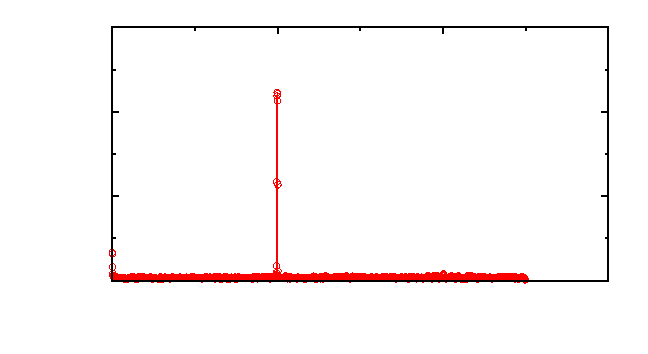
\includegraphics{power_250}}%
    \gplfronttext
  \end{picture}%
\endgroup
\caption{Ergebnis der Suche nach Störfrequenzen mit einer Abtastrate von \SI{250}{\hertz}. Die einzige erkennbare Störfrequenz liegt bei \SI{50}{\hertz} und wird durch das Stromnetz verursacht.}\label{fig:stoer}
\end{figure}
\\

\subsection{Temperaturmessungen}
Aus den Messungen der Temperatur als Funktion des Abstandes ergibt sich das in \cref{fig:temp-prof} dargestellte Temperaturprofil. Es ist sowohl das Ergebnis der Messung mit dem beweglichen Thermistor, als auch die Messung der Temperatur mit dem Thermistor-Array zu sehen. 
\cref{fig:temp-array} hingegen zeigt allein die Messung mit dem Thermistorarry.
\\
\begin{figure}
\centering
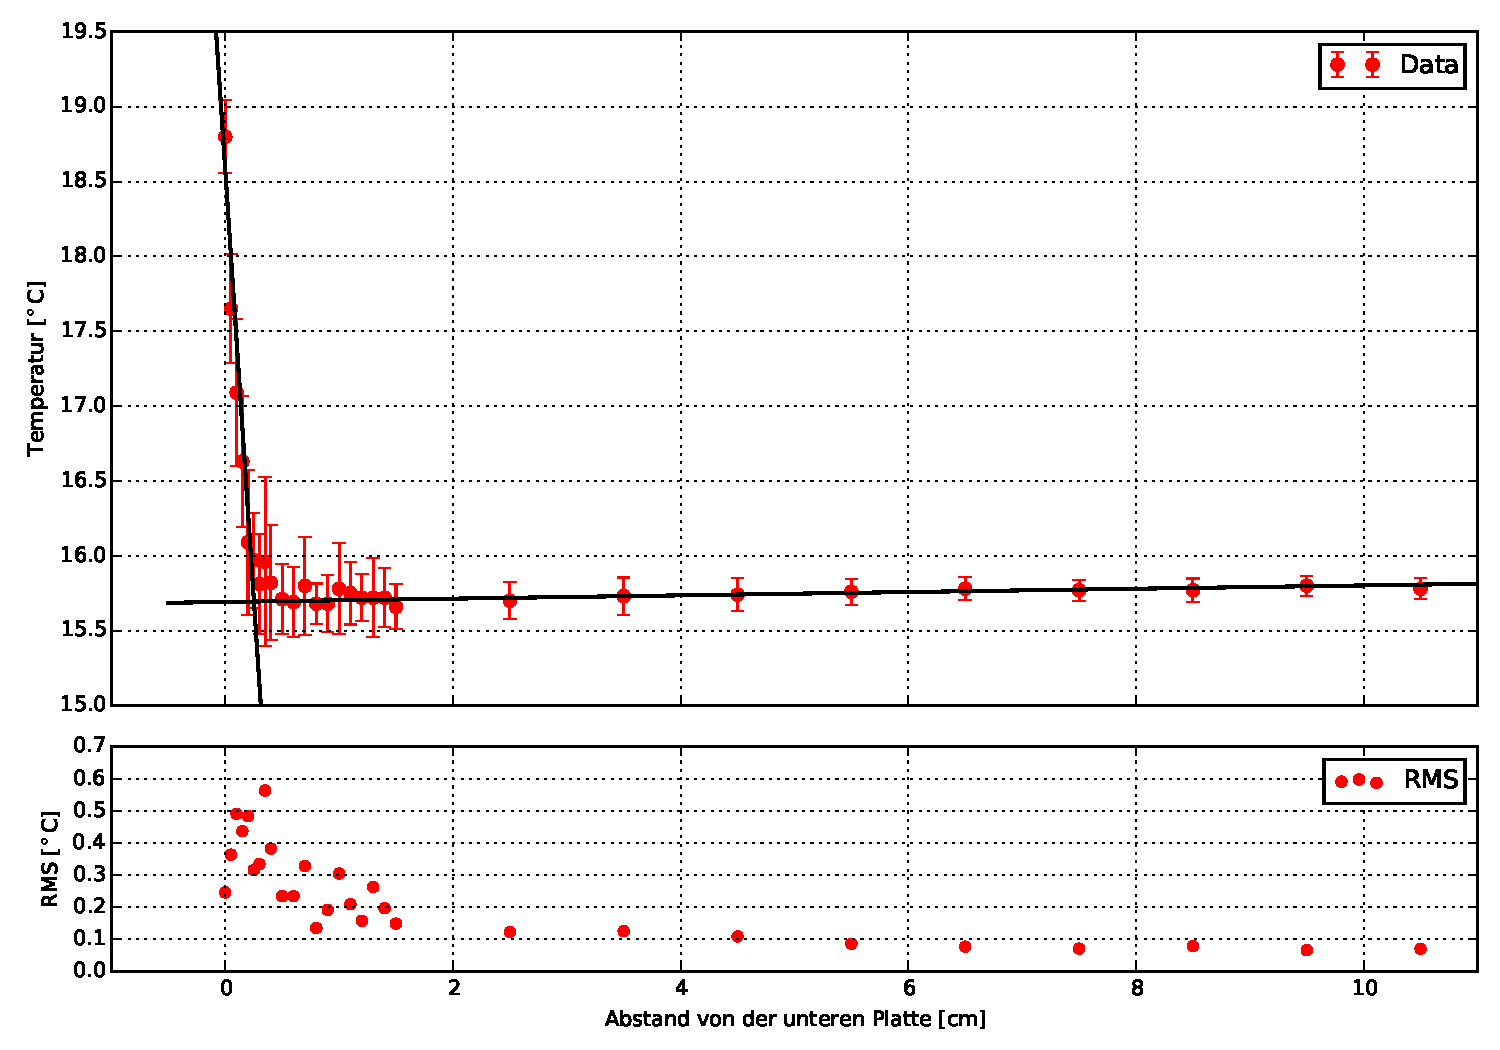
\includegraphics[width=\textwidth]{plots/T_profile2.pdf}
\caption{Temperaturprofil der unteren Hälfte der Zelle, als Funktion des Abstandes von der Heizplatte. Zu sehen ist die vollständige Messreihe mittels beweglichem Thermistor, und die ersten drei Messwerte des Thermistorarrays.
Zur Bestimmung der thermischen Grenzschicht wurde der Schnittpunkt zweier linearer Fits bestimmt.}\label{fig:temp-prof}
\end{figure}
Aus dem Temperaturprofil lässt sich die Nusseltzahl, über die thermische Grenzschicht bestimmen. Der bestimmte Schnittpunkt der beiden in \cref{fig:temp-prof} zu sehenden Fits liegt bei einem Abstand von \SI{0.25\pm0.4}{\centi\meter}. Nach \cref{eq:nusselt} ergibt sich dies zu einer Nusseltzahl von $\text{Nu}=\SI{40\pm7}{}$.
\\
\begin{figure}
	\centering
	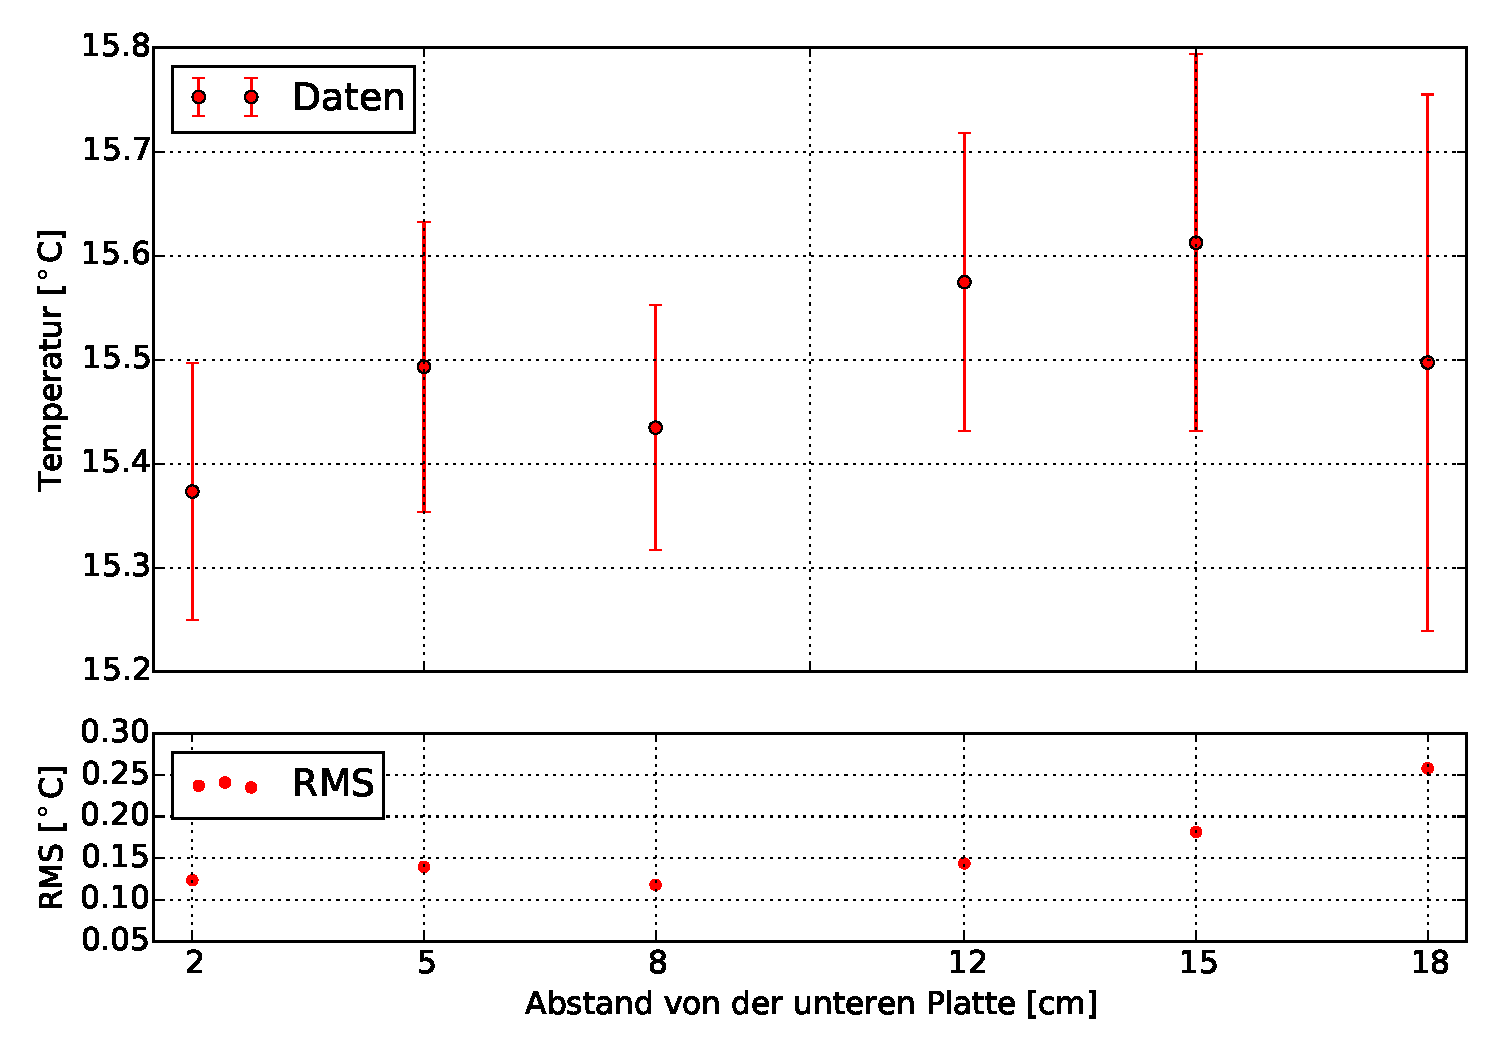
\includegraphics[width=\textwidth]{plots/T_korr_profile.pdf}
	\caption{Messungen des Temperaturprofils mithilfe des Thermistorarrays. Zu sehen sind die Mittelwerte der 30-stündigen Messung, für jeden Thermistor bzw. seine Position.}\label{fig:temp-array}
\end{figure}
Die in \cref{fig:temp-prof, fig:temp-array} dargestellten Profile lassen sich mit den aus der Simulation gewonnenen Profilen für unterschiedliche Rayleighzahlen vergleichen.
Diese sind in \cref{fig:sim-temp} dargestellt.
\\
\begin{figure}
	\centering
	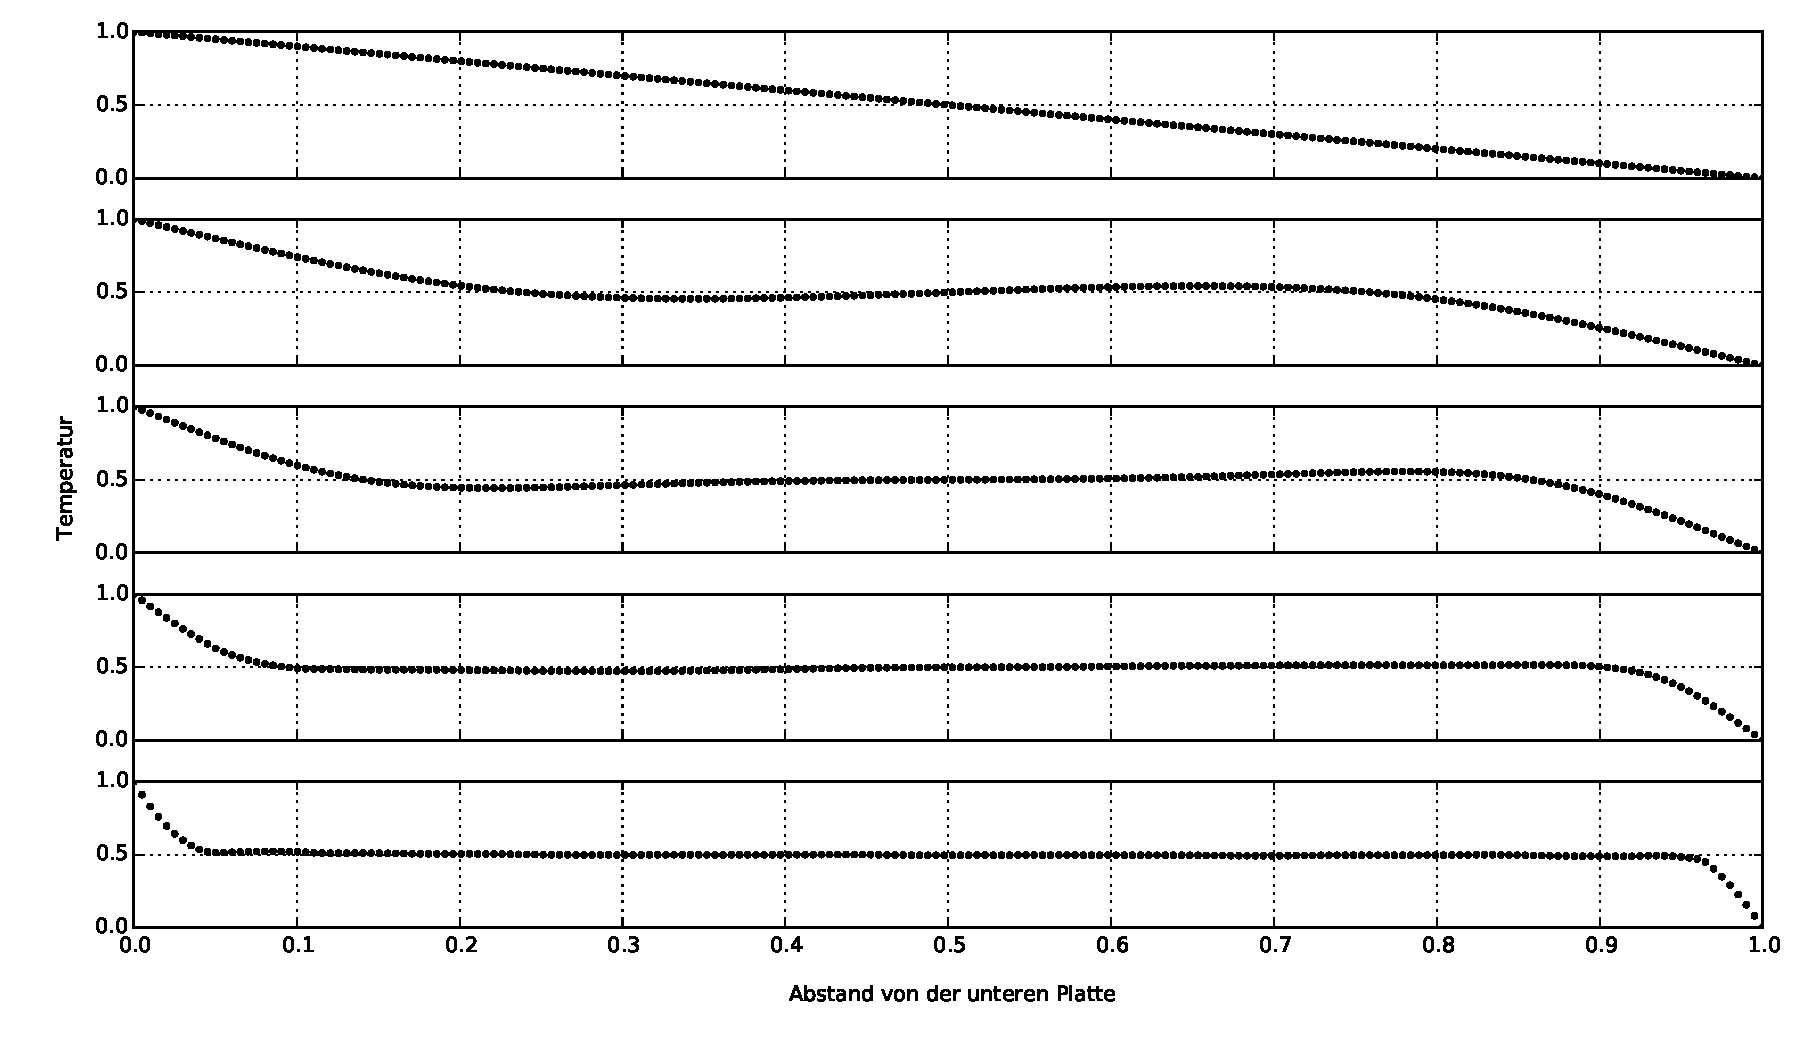
\includegraphics[width=\textwidth]{plots/T_sim_Profile.pdf}
	\caption{Temperaturprofile einer Rayleigh-Benard-Zelle zu verschiedenen Rayleighzahlen.}\label{fig:sim-temp}
\end{figure}
Für die 30-stündige Messung ist es interessant die Verteilung der Messwerte zu betrachten. \cref{fig:hist} zeigt Histogramme der gemessenen Werte über die gesamte Messreihe hinweg. Man erkennt, dass das Maximum der Verteilungen für jeden Thermistor in etwa bei der gleichen Temperatur \SI{15.5}{\celsius} liegt. 
Allerdings kommt es durch die Nähe zur Heiz- bzw. Kühlplatte zu häufigen Messung von Temperaturen mit einer starken Abweichung vom Maximum.
Der Thermistor in der Nähe der Heizplatte misst häufiger Temperaturen über der Durchschnittstemperatur, während beim Thermistor an der Kühlplatte häufiger niederigere Temperaturen gemessen werden.
Dieser Effekt lässt sich abgeschwächt auch in den weiter entfernten Thermistoren erkennen.
\begin{figure}
	\centering
	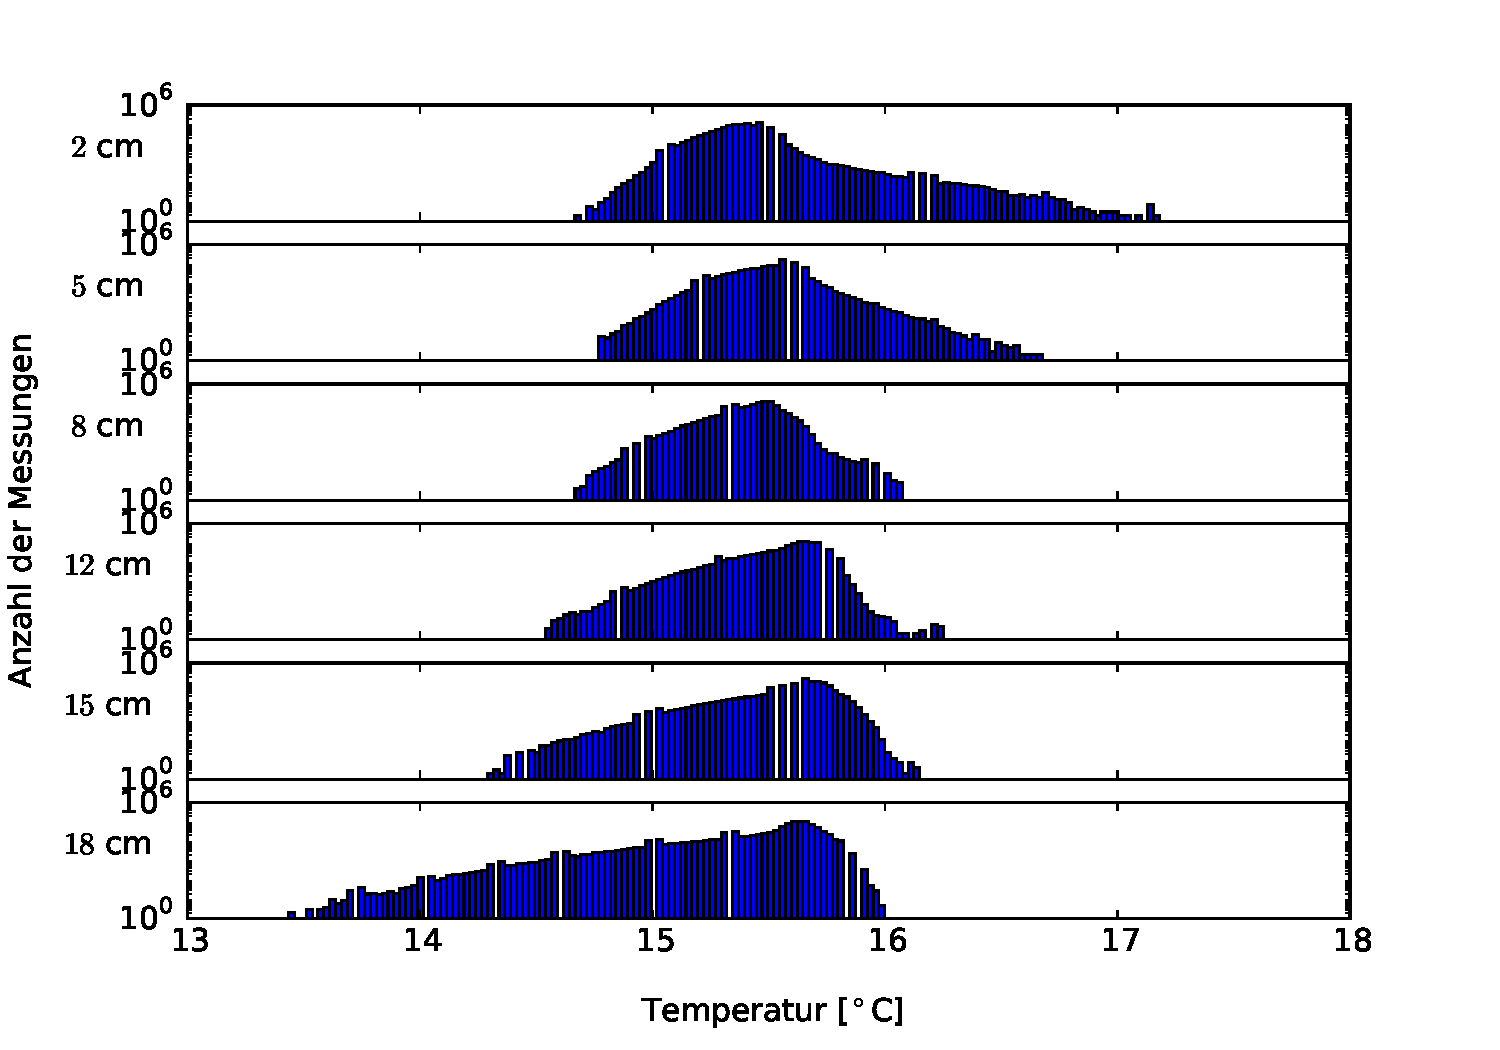
\includegraphics[width=\textwidth]{plots/T_hist.pdf}\caption{Verteilung der Messwerte der einzelnen Thermistoren als Funktion der Temperatur. Der Abstand bezeichnet den Abstand von der Heizplatte. Die Histogramme sind auf einer logarithmischen Skala aufgetragen. Bei den Lücken in den Histogrammen, handelt es sich um Fehler, die Messwerte aus diesen Boxen auf die benachbarten Boxen verteilen.}\label{fig:hist}
\end{figure}

\subsection{Geschwindigkeitsprofile}
Über die Messung der Temperatur mit dem beweglichen Thermistor lässt sich das Geschwindigkeitsprofil der Zelle ermitteln.
Dazu wird ausgenutzt, dass entstehende Plumes in etwa dem Verlauf der Konvektionswalze folgen, und in erster Näherung die gleiche Geschwindigkeit besitzen.
\\
In der mit dem Thermistor an einer Höhe aufgenommenen Zeitreihe sind Plumes als ein vorübergehender Anstieg bzw. Abfall der Temperatur zu erkennen. 
Die Geschwindigkeit des Plumes ist invers proportional zur Breite der Senke bzw. des Hügels.
Diese ist wiederum charakterisiert, durch die Frequenzzusammensetzung des Plumes im Fourierraum.
In \cref{fig:abbruch} ist eindeutig die größte Frequenz des Plume-Bündels zu erkennen. Diese Abbruchfrequenz ist direkt proportional zur durchschnittlichen Geschwindigkeit der Plumes in diesem Abstand von der Heizplatte.
\\
Das Geschwindigkeitsprofil der unteren \SI{10}{\centi\meter} ist in in \cref{fig:vprof_freq} zu sehen. 
Das Profil der Abbruchfrequenzen $f_c$ entspricht hier dem Verlauf des Geschwindigkeitsprofils.
Der lineare Fit der ersten Werte zeigt, dass selbst an der Heizplatte eine Geschwindigkeit zu Messen ist.
\\
\begin{figure}
	% GNUPLOT: LaTeX picture with Postscript
\begingroup
  \makeatletter
  \providecommand\color[2][]{%
    \GenericError{(gnuplot) \space\space\space\@spaces}{%
      Package color not loaded in conjunction with
      terminal option `colourtext'%
    }{See the gnuplot documentation for explanation.%
    }{Either use 'blacktext' in gnuplot or load the package
      color.sty in LaTeX.}%
    \renewcommand\color[2][]{}%
  }%
  \providecommand\includegraphics[2][]{%
    \GenericError{(gnuplot) \space\space\space\@spaces}{%
      Package graphicx or graphics not loaded%
    }{See the gnuplot documentation for explanation.%
    }{The gnuplot epslatex terminal needs graphicx.sty or graphics.sty.}%
    \renewcommand\includegraphics[2][]{}%
  }%
  \providecommand\rotatebox[2]{#2}%
  \@ifundefined{ifGPcolor}{%
    \newif\ifGPcolor
    \GPcolortrue
  }{}%
  \@ifundefined{ifGPblacktext}{%
    \newif\ifGPblacktext
    \GPblacktexttrue
  }{}%
  % define a \g@addto@macro without @ in the name:
  \let\gplgaddtomacro\g@addto@macro
  % define empty templates for all commands taking text:
  \gdef\gplbacktext{}%
  \gdef\gplfronttext{}%
  \makeatother
  \ifGPblacktext
    % no textcolor at all
    \def\colorrgb#1{}%
    \def\colorgray#1{}%
  \else
    % gray or color?
    \ifGPcolor
      \def\colorrgb#1{\color[rgb]{#1}}%
      \def\colorgray#1{\color[gray]{#1}}%
      \expandafter\def\csname LTw\endcsname{\color{white}}%
      \expandafter\def\csname LTb\endcsname{\color{black}}%
      \expandafter\def\csname LTa\endcsname{\color{black}}%
      \expandafter\def\csname LT0\endcsname{\color[rgb]{1,0,0}}%
      \expandafter\def\csname LT1\endcsname{\color[rgb]{0,1,0}}%
      \expandafter\def\csname LT2\endcsname{\color[rgb]{0,0,1}}%
      \expandafter\def\csname LT3\endcsname{\color[rgb]{1,0,1}}%
      \expandafter\def\csname LT4\endcsname{\color[rgb]{0,1,1}}%
      \expandafter\def\csname LT5\endcsname{\color[rgb]{1,1,0}}%
      \expandafter\def\csname LT6\endcsname{\color[rgb]{0,0,0}}%
      \expandafter\def\csname LT7\endcsname{\color[rgb]{1,0.3,0}}%
      \expandafter\def\csname LT8\endcsname{\color[rgb]{0.5,0.5,0.5}}%
    \else
      % gray
      \def\colorrgb#1{\color{black}}%
      \def\colorgray#1{\color[gray]{#1}}%
      \expandafter\def\csname LTw\endcsname{\color{white}}%
      \expandafter\def\csname LTb\endcsname{\color{black}}%
      \expandafter\def\csname LTa\endcsname{\color{black}}%
      \expandafter\def\csname LT0\endcsname{\color{black}}%
      \expandafter\def\csname LT1\endcsname{\color{black}}%
      \expandafter\def\csname LT2\endcsname{\color{black}}%
      \expandafter\def\csname LT3\endcsname{\color{black}}%
      \expandafter\def\csname LT4\endcsname{\color{black}}%
      \expandafter\def\csname LT5\endcsname{\color{black}}%
      \expandafter\def\csname LT6\endcsname{\color{black}}%
      \expandafter\def\csname LT7\endcsname{\color{black}}%
      \expandafter\def\csname LT8\endcsname{\color{black}}%
    \fi
  \fi
  \setlength{\unitlength}{0.0500bp}%
  \begin{picture}(5668.00,3400.00)%
    \gplgaddtomacro\gplbacktext{%
      \csname LTb\endcsname%
      \put(946,704){\makebox(0,0)[r]{\strut{}$10^{-3}$}}%
      \put(946,1312){\makebox(0,0)[r]{\strut{}$10^{-2}$}}%
      \put(946,1920){\makebox(0,0)[r]{\strut{}$10^{-1}$}}%
      \put(946,2527){\makebox(0,0)[r]{\strut{}$10^{0}$}}%
      \put(946,3135){\makebox(0,0)[r]{\strut{}$10^{1}$}}%
      \put(1078,484){\makebox(0,0){\strut{}$10^{-2}$}}%
      \put(2476,484){\makebox(0,0){\strut{}$10^{-1}$}}%
      \put(3873,484){\makebox(0,0){\strut{}$10^{0}$}}%
      \put(5271,484){\makebox(0,0){\strut{}$10^{1}$}}%
      \put(176,1919){\rotatebox{-270}{\makebox(0,0){\strut{}Häufigkeit}}}%
      \put(3174,154){\makebox(0,0){\strut{}Frequenz~[\si{\hertz}]}}%
      \put(3453,2527){\makebox(0,0)[l]{\strut{}$f_c$}}%
    }%
    \gplgaddtomacro\gplfronttext{%
    }%
    \gplbacktext
    \put(0,0){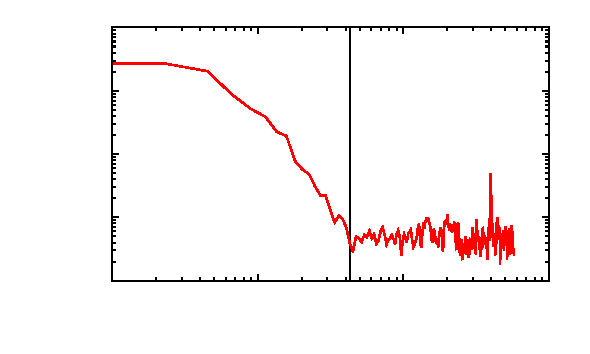
\includegraphics{power_0000}}%
    \gplfronttext
  \end{picture}%
\endgroup
\caption{Ermittlung der Abbruchfrequenz einer Messung. Dieses Beispiel zeigt die Bestimmung der Abbruchfrequenz für die Messung der Temperatur in unmittelbarer Nähe der Platte. }\label{fig:abbruch}
\end{figure}
\begin{figure}
	% GNUPLOT: LaTeX picture with Postscript
\begingroup
  \makeatletter
  \providecommand\color[2][]{%
    \GenericError{(gnuplot) \space\space\space\@spaces}{%
      Package color not loaded in conjunction with
      terminal option `colourtext'%
    }{See the gnuplot documentation for explanation.%
    }{Either use 'blacktext' in gnuplot or load the package
      color.sty in LaTeX.}%
    \renewcommand\color[2][]{}%
  }%
  \providecommand\includegraphics[2][]{%
    \GenericError{(gnuplot) \space\space\space\@spaces}{%
      Package graphicx or graphics not loaded%
    }{See the gnuplot documentation for explanation.%
    }{The gnuplot epslatex terminal needs graphicx.sty or graphics.sty.}%
    \renewcommand\includegraphics[2][]{}%
  }%
  \providecommand\rotatebox[2]{#2}%
  \@ifundefined{ifGPcolor}{%
    \newif\ifGPcolor
    \GPcolortrue
  }{}%
  \@ifundefined{ifGPblacktext}{%
    \newif\ifGPblacktext
    \GPblacktexttrue
  }{}%
  % define a \g@addto@macro without @ in the name:
  \let\gplgaddtomacro\g@addto@macro
  % define empty templates for all commands taking text:
  \gdef\gplbacktext{}%
  \gdef\gplfronttext{}%
  \makeatother
  \ifGPblacktext
    % no textcolor at all
    \def\colorrgb#1{}%
    \def\colorgray#1{}%
  \else
    % gray or color?
    \ifGPcolor
      \def\colorrgb#1{\color[rgb]{#1}}%
      \def\colorgray#1{\color[gray]{#1}}%
      \expandafter\def\csname LTw\endcsname{\color{white}}%
      \expandafter\def\csname LTb\endcsname{\color{black}}%
      \expandafter\def\csname LTa\endcsname{\color{black}}%
      \expandafter\def\csname LT0\endcsname{\color[rgb]{1,0,0}}%
      \expandafter\def\csname LT1\endcsname{\color[rgb]{0,1,0}}%
      \expandafter\def\csname LT2\endcsname{\color[rgb]{0,0,1}}%
      \expandafter\def\csname LT3\endcsname{\color[rgb]{1,0,1}}%
      \expandafter\def\csname LT4\endcsname{\color[rgb]{0,1,1}}%
      \expandafter\def\csname LT5\endcsname{\color[rgb]{1,1,0}}%
      \expandafter\def\csname LT6\endcsname{\color[rgb]{0,0,0}}%
      \expandafter\def\csname LT7\endcsname{\color[rgb]{1,0.3,0}}%
      \expandafter\def\csname LT8\endcsname{\color[rgb]{0.5,0.5,0.5}}%
    \else
      % gray
      \def\colorrgb#1{\color{black}}%
      \def\colorgray#1{\color[gray]{#1}}%
      \expandafter\def\csname LTw\endcsname{\color{white}}%
      \expandafter\def\csname LTb\endcsname{\color{black}}%
      \expandafter\def\csname LTa\endcsname{\color{black}}%
      \expandafter\def\csname LT0\endcsname{\color{black}}%
      \expandafter\def\csname LT1\endcsname{\color{black}}%
      \expandafter\def\csname LT2\endcsname{\color{black}}%
      \expandafter\def\csname LT3\endcsname{\color{black}}%
      \expandafter\def\csname LT4\endcsname{\color{black}}%
      \expandafter\def\csname LT5\endcsname{\color{black}}%
      \expandafter\def\csname LT6\endcsname{\color{black}}%
      \expandafter\def\csname LT7\endcsname{\color{black}}%
      \expandafter\def\csname LT8\endcsname{\color{black}}%
    \fi
  \fi
  \setlength{\unitlength}{0.0500bp}%
  \begin{picture}(7936.00,4534.00)%
    \gplgaddtomacro\gplbacktext{%
      \csname LTb\endcsname%
      \put(946,704){\makebox(0,0)[r]{\strut{} 0}}%
      \put(946,1417){\makebox(0,0)[r]{\strut{} 0.2}}%
      \put(946,2130){\makebox(0,0)[r]{\strut{} 0.4}}%
      \put(946,2843){\makebox(0,0)[r]{\strut{} 0.6}}%
      \put(946,3556){\makebox(0,0)[r]{\strut{} 0.8}}%
      \put(946,4269){\makebox(0,0)[r]{\strut{} 1}}%
      \put(1336,484){\makebox(0,0){\strut{} 0}}%
      \put(2887,484){\makebox(0,0){\strut{} 3}}%
      \put(4438,484){\makebox(0,0){\strut{} 6}}%
      \put(5988,484){\makebox(0,0){\strut{} 9}}%
      \put(7539,484){\makebox(0,0){\strut{} 12}}%
      \put(176,2486){\rotatebox{-270}{\makebox(0,0){\strut{}$f_c~[\si{\hertz}]$}}}%
      \put(4308,154){\makebox(0,0){\strut{}Abstand von der Heizplatte~[\si{\centi\meter}]}}%
    }%
    \gplgaddtomacro\gplfronttext{%
    }%
    \gplgaddtomacro\gplbacktext{%
      \csname LTb\endcsname%
      \put(4297,2740){\makebox(0,0)[r]{\strut{} 0.5}}%
      \put(4297,4042){\makebox(0,0)[r]{\strut{} 1}}%
      \put(4667,2260){\makebox(0,0){\strut{} 0}}%
      \put(5857,2260){\makebox(0,0){\strut{} 0.5}}%
      \put(7047,2260){\makebox(0,0){\strut{} 1}}%
    }%
    \gplgaddtomacro\gplfronttext{%
    }%
    \gplbacktext
    \put(0,0){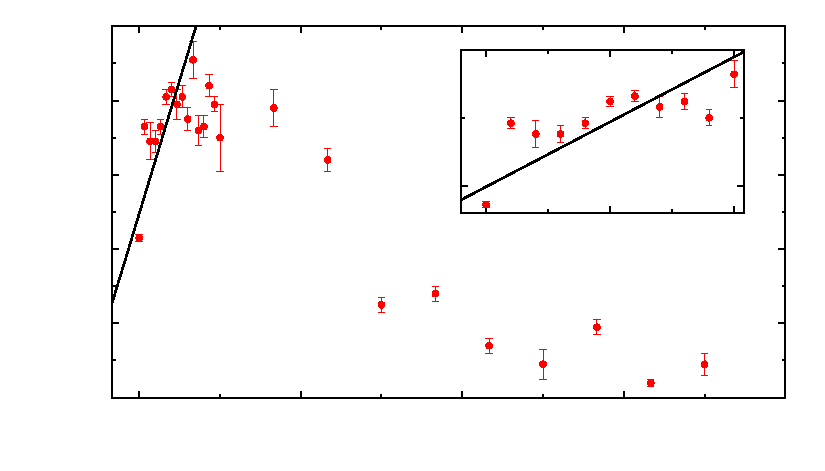
\includegraphics{v_prof_fc}}%
    \gplfronttext
  \end{picture}%
\endgroup
\caption{Zu sehen ist die Abhängigkeit der Abbruchfrequenz $f_c$ in Abhängigkeit von dem Abstand von der Heizplatte. Dieser Verlauf entspricht auch dem Geschwindigkeitsprofil in der Zelle, da die Geschwindigkeit proportional zur Abbruchfrequenz ist.}\label{fig:vprof_freq}
\end{figure}
Aus der 30-stündigen Messung lässt sich die Geschwindigkeit an fünf Stellen der Zelle bestimmen. Dazu wird aus den Temperaturmesswerten die Korrelation jeweils zweier Thermistoren gebildet.
Die Zeit $\tau$ des Maximums einer Korrelation entspricht der mittleren Zeit, die ein Plume braucht um von einem Thermistor zum anderen zu 


%\begin{figure}
%
%\end{figure}
\begin{figure}[!h]
        \centering
        \begin{subfigure}{0.5\textwidth}
        % GNUPLOT: LaTeX picture with Postscript
\begingroup
  \makeatletter
  \providecommand\color[2][]{%
    \GenericError{(gnuplot) \space\space\space\@spaces}{%
      Package color not loaded in conjunction with
      terminal option `colourtext'%
    }{See the gnuplot documentation for explanation.%
    }{Either use 'blacktext' in gnuplot or load the package
      color.sty in LaTeX.}%
    \renewcommand\color[2][]{}%
  }%
  \providecommand\includegraphics[2][]{%
    \GenericError{(gnuplot) \space\space\space\@spaces}{%
      Package graphicx or graphics not loaded%
    }{See the gnuplot documentation for explanation.%
    }{The gnuplot epslatex terminal needs graphicx.sty or graphics.sty.}%
    \renewcommand\includegraphics[2][]{}%
  }%
  \providecommand\rotatebox[2]{#2}%
  \@ifundefined{ifGPcolor}{%
    \newif\ifGPcolor
    \GPcolortrue
  }{}%
  \@ifundefined{ifGPblacktext}{%
    \newif\ifGPblacktext
    \GPblacktexttrue
  }{}%
  % define a \g@addto@macro without @ in the name:
  \let\gplgaddtomacro\g@addto@macro
  % define empty templates for all commands taking text:
  \gdef\gplbacktext{}%
  \gdef\gplfronttext{}%
  \makeatother
  \ifGPblacktext
    % no textcolor at all
    \def\colorrgb#1{}%
    \def\colorgray#1{}%
  \else
    % gray or color?
    \ifGPcolor
      \def\colorrgb#1{\color[rgb]{#1}}%
      \def\colorgray#1{\color[gray]{#1}}%
      \expandafter\def\csname LTw\endcsname{\color{white}}%
      \expandafter\def\csname LTb\endcsname{\color{black}}%
      \expandafter\def\csname LTa\endcsname{\color{black}}%
      \expandafter\def\csname LT0\endcsname{\color[rgb]{1,0,0}}%
      \expandafter\def\csname LT1\endcsname{\color[rgb]{0,1,0}}%
      \expandafter\def\csname LT2\endcsname{\color[rgb]{0,0,1}}%
      \expandafter\def\csname LT3\endcsname{\color[rgb]{1,0,1}}%
      \expandafter\def\csname LT4\endcsname{\color[rgb]{0,1,1}}%
      \expandafter\def\csname LT5\endcsname{\color[rgb]{1,1,0}}%
      \expandafter\def\csname LT6\endcsname{\color[rgb]{0,0,0}}%
      \expandafter\def\csname LT7\endcsname{\color[rgb]{1,0.3,0}}%
      \expandafter\def\csname LT8\endcsname{\color[rgb]{0.5,0.5,0.5}}%
    \else
      % gray
      \def\colorrgb#1{\color{black}}%
      \def\colorgray#1{\color[gray]{#1}}%
      \expandafter\def\csname LTw\endcsname{\color{white}}%
      \expandafter\def\csname LTb\endcsname{\color{black}}%
      \expandafter\def\csname LTa\endcsname{\color{black}}%
      \expandafter\def\csname LT0\endcsname{\color{black}}%
      \expandafter\def\csname LT1\endcsname{\color{black}}%
      \expandafter\def\csname LT2\endcsname{\color{black}}%
      \expandafter\def\csname LT3\endcsname{\color{black}}%
      \expandafter\def\csname LT4\endcsname{\color{black}}%
      \expandafter\def\csname LT5\endcsname{\color{black}}%
      \expandafter\def\csname LT6\endcsname{\color{black}}%
      \expandafter\def\csname LT7\endcsname{\color{black}}%
      \expandafter\def\csname LT8\endcsname{\color{black}}%
    \fi
  \fi
  \setlength{\unitlength}{0.0500bp}%
  \begin{picture}(3968.00,3400.00)%
    \gplgaddtomacro\gplbacktext{%
      \csname LTb\endcsname%
      \put(1342,704){\makebox(0,0)[r]{\strut{} 0}}%
      \put(1342,1312){\makebox(0,0)[r]{\strut{} 0.0001}}%
      \put(1342,1920){\makebox(0,0)[r]{\strut{} 0.0002}}%
      \put(1342,2527){\makebox(0,0)[r]{\strut{} 0.0003}}%
      \put(1342,3135){\makebox(0,0)[r]{\strut{} 0.0004}}%
      \put(1474,484){\makebox(0,0){\strut{} 0}}%
      \put(2523,484){\makebox(0,0){\strut{} 0.5}}%
      \put(3571,484){\makebox(0,0){\strut{} 1}}%
      \put(176,1919){\rotatebox{-270}{\makebox(0,0){\strut{}Geschwindigkeit~[$\kappa/L$]}}}%
      \put(2522,154){\makebox(0,0){\strut{}$z$-Position~[$L$]}}%
    }%
    \gplgaddtomacro\gplfronttext{%
    }%
    \gplbacktext
    \put(0,0){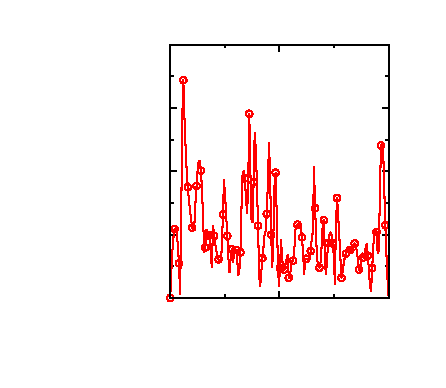
\includegraphics{v_prof_Ra_1e3}}%
    \gplfronttext
  \end{picture}%
\endgroup

        \caption{$\Ra = \num{e3}$}
        \label{fig:vprof_Ra_1e3}
\end{subfigure}\hfill
        \begin{subfigure}{0.5\textwidth}
        % GNUPLOT: LaTeX picture with Postscript
\begingroup
  \makeatletter
  \providecommand\color[2][]{%
    \GenericError{(gnuplot) \space\space\space\@spaces}{%
      Package color not loaded in conjunction with
      terminal option `colourtext'%
    }{See the gnuplot documentation for explanation.%
    }{Either use 'blacktext' in gnuplot or load the package
      color.sty in LaTeX.}%
    \renewcommand\color[2][]{}%
  }%
  \providecommand\includegraphics[2][]{%
    \GenericError{(gnuplot) \space\space\space\@spaces}{%
      Package graphicx or graphics not loaded%
    }{See the gnuplot documentation for explanation.%
    }{The gnuplot epslatex terminal needs graphicx.sty or graphics.sty.}%
    \renewcommand\includegraphics[2][]{}%
  }%
  \providecommand\rotatebox[2]{#2}%
  \@ifundefined{ifGPcolor}{%
    \newif\ifGPcolor
    \GPcolortrue
  }{}%
  \@ifundefined{ifGPblacktext}{%
    \newif\ifGPblacktext
    \GPblacktexttrue
  }{}%
  % define a \g@addto@macro without @ in the name:
  \let\gplgaddtomacro\g@addto@macro
  % define empty templates for all commands taking text:
  \gdef\gplbacktext{}%
  \gdef\gplfronttext{}%
  \makeatother
  \ifGPblacktext
    % no textcolor at all
    \def\colorrgb#1{}%
    \def\colorgray#1{}%
  \else
    % gray or color?
    \ifGPcolor
      \def\colorrgb#1{\color[rgb]{#1}}%
      \def\colorgray#1{\color[gray]{#1}}%
      \expandafter\def\csname LTw\endcsname{\color{white}}%
      \expandafter\def\csname LTb\endcsname{\color{black}}%
      \expandafter\def\csname LTa\endcsname{\color{black}}%
      \expandafter\def\csname LT0\endcsname{\color[rgb]{1,0,0}}%
      \expandafter\def\csname LT1\endcsname{\color[rgb]{0,1,0}}%
      \expandafter\def\csname LT2\endcsname{\color[rgb]{0,0,1}}%
      \expandafter\def\csname LT3\endcsname{\color[rgb]{1,0,1}}%
      \expandafter\def\csname LT4\endcsname{\color[rgb]{0,1,1}}%
      \expandafter\def\csname LT5\endcsname{\color[rgb]{1,1,0}}%
      \expandafter\def\csname LT6\endcsname{\color[rgb]{0,0,0}}%
      \expandafter\def\csname LT7\endcsname{\color[rgb]{1,0.3,0}}%
      \expandafter\def\csname LT8\endcsname{\color[rgb]{0.5,0.5,0.5}}%
    \else
      % gray
      \def\colorrgb#1{\color{black}}%
      \def\colorgray#1{\color[gray]{#1}}%
      \expandafter\def\csname LTw\endcsname{\color{white}}%
      \expandafter\def\csname LTb\endcsname{\color{black}}%
      \expandafter\def\csname LTa\endcsname{\color{black}}%
      \expandafter\def\csname LT0\endcsname{\color{black}}%
      \expandafter\def\csname LT1\endcsname{\color{black}}%
      \expandafter\def\csname LT2\endcsname{\color{black}}%
      \expandafter\def\csname LT3\endcsname{\color{black}}%
      \expandafter\def\csname LT4\endcsname{\color{black}}%
      \expandafter\def\csname LT5\endcsname{\color{black}}%
      \expandafter\def\csname LT6\endcsname{\color{black}}%
      \expandafter\def\csname LT7\endcsname{\color{black}}%
      \expandafter\def\csname LT8\endcsname{\color{black}}%
    \fi
  \fi
  \setlength{\unitlength}{0.0500bp}%
  \begin{picture}(3968.00,3400.00)%
    \gplgaddtomacro\gplbacktext{%
      \csname LTb\endcsname%
      \put(814,704){\makebox(0,0)[r]{\strut{} 0}}%
      \put(814,1190){\makebox(0,0)[r]{\strut{} 5}}%
      \put(814,1676){\makebox(0,0)[r]{\strut{} 10}}%
      \put(814,2163){\makebox(0,0)[r]{\strut{} 15}}%
      \put(814,2649){\makebox(0,0)[r]{\strut{} 20}}%
      \put(814,3135){\makebox(0,0)[r]{\strut{} 25}}%
      \put(946,484){\makebox(0,0){\strut{} 0}}%
      \put(2259,484){\makebox(0,0){\strut{} 0.5}}%
      \put(3571,484){\makebox(0,0){\strut{} 1}}%
      \put(176,1919){\rotatebox{-270}{\makebox(0,0){\strut{}Geschwindigkeit~[$\kappa/L$]}}}%
      \put(2258,154){\makebox(0,0){\strut{}$z$-Position~[$L$]}}%
    }%
    \gplgaddtomacro\gplfronttext{%
    }%
    \gplbacktext
    \put(0,0){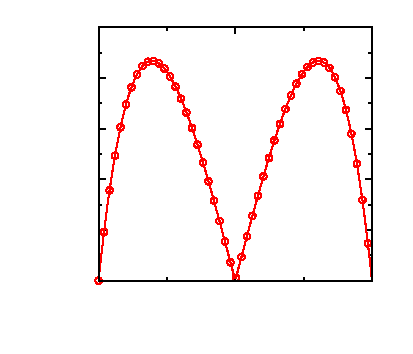
\includegraphics{v_prof_Ra_1e4}}%
    \gplfronttext
  \end{picture}%
\endgroup

        \caption{$\Ra = \num{e4}$}
        \label{fig:vprof_Ra_1e4}
\end{subfigure} \\
        \begin{subfigure}{0.5\textwidth}
        % GNUPLOT: LaTeX picture with Postscript
\begingroup
  \makeatletter
  \providecommand\color[2][]{%
    \GenericError{(gnuplot) \space\space\space\@spaces}{%
      Package color not loaded in conjunction with
      terminal option `colourtext'%
    }{See the gnuplot documentation for explanation.%
    }{Either use 'blacktext' in gnuplot or load the package
      color.sty in LaTeX.}%
    \renewcommand\color[2][]{}%
  }%
  \providecommand\includegraphics[2][]{%
    \GenericError{(gnuplot) \space\space\space\@spaces}{%
      Package graphicx or graphics not loaded%
    }{See the gnuplot documentation for explanation.%
    }{The gnuplot epslatex terminal needs graphicx.sty or graphics.sty.}%
    \renewcommand\includegraphics[2][]{}%
  }%
  \providecommand\rotatebox[2]{#2}%
  \@ifundefined{ifGPcolor}{%
    \newif\ifGPcolor
    \GPcolortrue
  }{}%
  \@ifundefined{ifGPblacktext}{%
    \newif\ifGPblacktext
    \GPblacktexttrue
  }{}%
  % define a \g@addto@macro without @ in the name:
  \let\gplgaddtomacro\g@addto@macro
  % define empty templates for all commands taking text:
  \gdef\gplbacktext{}%
  \gdef\gplfronttext{}%
  \makeatother
  \ifGPblacktext
    % no textcolor at all
    \def\colorrgb#1{}%
    \def\colorgray#1{}%
  \else
    % gray or color?
    \ifGPcolor
      \def\colorrgb#1{\color[rgb]{#1}}%
      \def\colorgray#1{\color[gray]{#1}}%
      \expandafter\def\csname LTw\endcsname{\color{white}}%
      \expandafter\def\csname LTb\endcsname{\color{black}}%
      \expandafter\def\csname LTa\endcsname{\color{black}}%
      \expandafter\def\csname LT0\endcsname{\color[rgb]{1,0,0}}%
      \expandafter\def\csname LT1\endcsname{\color[rgb]{0,1,0}}%
      \expandafter\def\csname LT2\endcsname{\color[rgb]{0,0,1}}%
      \expandafter\def\csname LT3\endcsname{\color[rgb]{1,0,1}}%
      \expandafter\def\csname LT4\endcsname{\color[rgb]{0,1,1}}%
      \expandafter\def\csname LT5\endcsname{\color[rgb]{1,1,0}}%
      \expandafter\def\csname LT6\endcsname{\color[rgb]{0,0,0}}%
      \expandafter\def\csname LT7\endcsname{\color[rgb]{1,0.3,0}}%
      \expandafter\def\csname LT8\endcsname{\color[rgb]{0.5,0.5,0.5}}%
    \else
      % gray
      \def\colorrgb#1{\color{black}}%
      \def\colorgray#1{\color[gray]{#1}}%
      \expandafter\def\csname LTw\endcsname{\color{white}}%
      \expandafter\def\csname LTb\endcsname{\color{black}}%
      \expandafter\def\csname LTa\endcsname{\color{black}}%
      \expandafter\def\csname LT0\endcsname{\color{black}}%
      \expandafter\def\csname LT1\endcsname{\color{black}}%
      \expandafter\def\csname LT2\endcsname{\color{black}}%
      \expandafter\def\csname LT3\endcsname{\color{black}}%
      \expandafter\def\csname LT4\endcsname{\color{black}}%
      \expandafter\def\csname LT5\endcsname{\color{black}}%
      \expandafter\def\csname LT6\endcsname{\color{black}}%
      \expandafter\def\csname LT7\endcsname{\color{black}}%
      \expandafter\def\csname LT8\endcsname{\color{black}}%
    \fi
  \fi
  \setlength{\unitlength}{0.0500bp}%
  \begin{picture}(3968.00,3400.00)%
    \gplgaddtomacro\gplbacktext{%
      \csname LTb\endcsname%
      \put(814,704){\makebox(0,0)[r]{\strut{} 0}}%
      \put(814,1312){\makebox(0,0)[r]{\strut{} 20}}%
      \put(814,1920){\makebox(0,0)[r]{\strut{} 40}}%
      \put(814,2527){\makebox(0,0)[r]{\strut{} 60}}%
      \put(814,3135){\makebox(0,0)[r]{\strut{} 80}}%
      \put(946,484){\makebox(0,0){\strut{} 0}}%
      \put(2259,484){\makebox(0,0){\strut{} 0.5}}%
      \put(3571,484){\makebox(0,0){\strut{} 1}}%
      \put(176,1919){\rotatebox{-270}{\makebox(0,0){\strut{}Geschwindigkeit~[$\kappa/L$]}}}%
      \put(2258,154){\makebox(0,0){\strut{}$z$-Position~[$L$]}}%
    }%
    \gplgaddtomacro\gplfronttext{%
    }%
    \gplbacktext
    \put(0,0){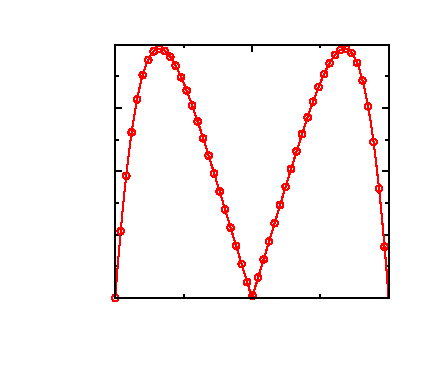
\includegraphics{v_prof_Ra_1e5}}%
    \gplfronttext
  \end{picture}%
\endgroup

        \caption{$\Ra = \num{e5}$}
        \label{fig:vprof_Ra_1e5}
\end{subfigure}\hfill
        \begin{subfigure}{0.5\textwidth}
        % GNUPLOT: LaTeX picture with Postscript
\begingroup
  \makeatletter
  \providecommand\color[2][]{%
    \GenericError{(gnuplot) \space\space\space\@spaces}{%
      Package color not loaded in conjunction with
      terminal option `colourtext'%
    }{See the gnuplot documentation for explanation.%
    }{Either use 'blacktext' in gnuplot or load the package
      color.sty in LaTeX.}%
    \renewcommand\color[2][]{}%
  }%
  \providecommand\includegraphics[2][]{%
    \GenericError{(gnuplot) \space\space\space\@spaces}{%
      Package graphicx or graphics not loaded%
    }{See the gnuplot documentation for explanation.%
    }{The gnuplot epslatex terminal needs graphicx.sty or graphics.sty.}%
    \renewcommand\includegraphics[2][]{}%
  }%
  \providecommand\rotatebox[2]{#2}%
  \@ifundefined{ifGPcolor}{%
    \newif\ifGPcolor
    \GPcolortrue
  }{}%
  \@ifundefined{ifGPblacktext}{%
    \newif\ifGPblacktext
    \GPblacktexttrue
  }{}%
  % define a \g@addto@macro without @ in the name:
  \let\gplgaddtomacro\g@addto@macro
  % define empty templates for all commands taking text:
  \gdef\gplbacktext{}%
  \gdef\gplfronttext{}%
  \makeatother
  \ifGPblacktext
    % no textcolor at all
    \def\colorrgb#1{}%
    \def\colorgray#1{}%
  \else
    % gray or color?
    \ifGPcolor
      \def\colorrgb#1{\color[rgb]{#1}}%
      \def\colorgray#1{\color[gray]{#1}}%
      \expandafter\def\csname LTw\endcsname{\color{white}}%
      \expandafter\def\csname LTb\endcsname{\color{black}}%
      \expandafter\def\csname LTa\endcsname{\color{black}}%
      \expandafter\def\csname LT0\endcsname{\color[rgb]{1,0,0}}%
      \expandafter\def\csname LT1\endcsname{\color[rgb]{0,1,0}}%
      \expandafter\def\csname LT2\endcsname{\color[rgb]{0,0,1}}%
      \expandafter\def\csname LT3\endcsname{\color[rgb]{1,0,1}}%
      \expandafter\def\csname LT4\endcsname{\color[rgb]{0,1,1}}%
      \expandafter\def\csname LT5\endcsname{\color[rgb]{1,1,0}}%
      \expandafter\def\csname LT6\endcsname{\color[rgb]{0,0,0}}%
      \expandafter\def\csname LT7\endcsname{\color[rgb]{1,0.3,0}}%
      \expandafter\def\csname LT8\endcsname{\color[rgb]{0.5,0.5,0.5}}%
    \else
      % gray
      \def\colorrgb#1{\color{black}}%
      \def\colorgray#1{\color[gray]{#1}}%
      \expandafter\def\csname LTw\endcsname{\color{white}}%
      \expandafter\def\csname LTb\endcsname{\color{black}}%
      \expandafter\def\csname LTa\endcsname{\color{black}}%
      \expandafter\def\csname LT0\endcsname{\color{black}}%
      \expandafter\def\csname LT1\endcsname{\color{black}}%
      \expandafter\def\csname LT2\endcsname{\color{black}}%
      \expandafter\def\csname LT3\endcsname{\color{black}}%
      \expandafter\def\csname LT4\endcsname{\color{black}}%
      \expandafter\def\csname LT5\endcsname{\color{black}}%
      \expandafter\def\csname LT6\endcsname{\color{black}}%
      \expandafter\def\csname LT7\endcsname{\color{black}}%
      \expandafter\def\csname LT8\endcsname{\color{black}}%
    \fi
  \fi
  \setlength{\unitlength}{0.0500bp}%
  \begin{picture}(3968.00,3400.00)%
    \gplgaddtomacro\gplbacktext{%
      \csname LTb\endcsname%
      \put(946,704){\makebox(0,0)[r]{\strut{} 0}}%
      \put(946,1514){\makebox(0,0)[r]{\strut{} 100}}%
      \put(946,2325){\makebox(0,0)[r]{\strut{} 200}}%
      \put(946,3135){\makebox(0,0)[r]{\strut{} 300}}%
      \put(1078,484){\makebox(0,0){\strut{} 0}}%
      \put(2325,484){\makebox(0,0){\strut{} 0.5}}%
      \put(3571,484){\makebox(0,0){\strut{} 1}}%
      \put(176,1919){\rotatebox{-270}{\makebox(0,0){\strut{}Geschwindigkeit~[$\kappa/L$]}}}%
      \put(2324,154){\makebox(0,0){\strut{}$z$-Position~[$L$]}}%
    }%
    \gplgaddtomacro\gplfronttext{%
    }%
    \gplbacktext
    \put(0,0){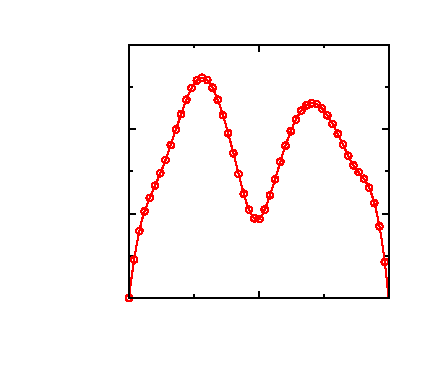
\includegraphics{v_prof_Ra_1e6}}%
    \gplfronttext
  \end{picture}%
\endgroup

        \caption{$\Ra = \num{e6}$}
        \label{fig:vprof_Ra_1e6}
\end{subfigure} \\
        \begin{subfigure}{0.5\textwidth}
        % GNUPLOT: LaTeX picture with Postscript
\begingroup
  \makeatletter
  \providecommand\color[2][]{%
    \GenericError{(gnuplot) \space\space\space\@spaces}{%
      Package color not loaded in conjunction with
      terminal option `colourtext'%
    }{See the gnuplot documentation for explanation.%
    }{Either use 'blacktext' in gnuplot or load the package
      color.sty in LaTeX.}%
    \renewcommand\color[2][]{}%
  }%
  \providecommand\includegraphics[2][]{%
    \GenericError{(gnuplot) \space\space\space\@spaces}{%
      Package graphicx or graphics not loaded%
    }{See the gnuplot documentation for explanation.%
    }{The gnuplot epslatex terminal needs graphicx.sty or graphics.sty.}%
    \renewcommand\includegraphics[2][]{}%
  }%
  \providecommand\rotatebox[2]{#2}%
  \@ifundefined{ifGPcolor}{%
    \newif\ifGPcolor
    \GPcolortrue
  }{}%
  \@ifundefined{ifGPblacktext}{%
    \newif\ifGPblacktext
    \GPblacktexttrue
  }{}%
  % define a \g@addto@macro without @ in the name:
  \let\gplgaddtomacro\g@addto@macro
  % define empty templates for all commands taking text:
  \gdef\gplbacktext{}%
  \gdef\gplfronttext{}%
  \makeatother
  \ifGPblacktext
    % no textcolor at all
    \def\colorrgb#1{}%
    \def\colorgray#1{}%
  \else
    % gray or color?
    \ifGPcolor
      \def\colorrgb#1{\color[rgb]{#1}}%
      \def\colorgray#1{\color[gray]{#1}}%
      \expandafter\def\csname LTw\endcsname{\color{white}}%
      \expandafter\def\csname LTb\endcsname{\color{black}}%
      \expandafter\def\csname LTa\endcsname{\color{black}}%
      \expandafter\def\csname LT0\endcsname{\color[rgb]{1,0,0}}%
      \expandafter\def\csname LT1\endcsname{\color[rgb]{0,1,0}}%
      \expandafter\def\csname LT2\endcsname{\color[rgb]{0,0,1}}%
      \expandafter\def\csname LT3\endcsname{\color[rgb]{1,0,1}}%
      \expandafter\def\csname LT4\endcsname{\color[rgb]{0,1,1}}%
      \expandafter\def\csname LT5\endcsname{\color[rgb]{1,1,0}}%
      \expandafter\def\csname LT6\endcsname{\color[rgb]{0,0,0}}%
      \expandafter\def\csname LT7\endcsname{\color[rgb]{1,0.3,0}}%
      \expandafter\def\csname LT8\endcsname{\color[rgb]{0.5,0.5,0.5}}%
    \else
      % gray
      \def\colorrgb#1{\color{black}}%
      \def\colorgray#1{\color[gray]{#1}}%
      \expandafter\def\csname LTw\endcsname{\color{white}}%
      \expandafter\def\csname LTb\endcsname{\color{black}}%
      \expandafter\def\csname LTa\endcsname{\color{black}}%
      \expandafter\def\csname LT0\endcsname{\color{black}}%
      \expandafter\def\csname LT1\endcsname{\color{black}}%
      \expandafter\def\csname LT2\endcsname{\color{black}}%
      \expandafter\def\csname LT3\endcsname{\color{black}}%
      \expandafter\def\csname LT4\endcsname{\color{black}}%
      \expandafter\def\csname LT5\endcsname{\color{black}}%
      \expandafter\def\csname LT6\endcsname{\color{black}}%
      \expandafter\def\csname LT7\endcsname{\color{black}}%
      \expandafter\def\csname LT8\endcsname{\color{black}}%
    \fi
  \fi
  \setlength{\unitlength}{0.0500bp}%
  \begin{picture}(3968.00,3400.00)%
    \gplgaddtomacro\gplbacktext{%
      \csname LTb\endcsname%
      \put(1078,704){\makebox(0,0)[r]{\strut{} 0}}%
      \put(1078,1514){\makebox(0,0)[r]{\strut{} 400}}%
      \put(1078,2325){\makebox(0,0)[r]{\strut{} 800}}%
      \put(1078,3135){\makebox(0,0)[r]{\strut{} 1200}}%
      \put(1210,484){\makebox(0,0){\strut{} 0}}%
      \put(2391,484){\makebox(0,0){\strut{} 0.5}}%
      \put(3571,484){\makebox(0,0){\strut{} 1}}%
      \put(176,1919){\rotatebox{-270}{\makebox(0,0){\strut{}Geschwindigkeit~[$\kappa/L$]}}}%
      \put(2390,154){\makebox(0,0){\strut{}$z$-Position~[$L$]}}%
    }%
    \gplgaddtomacro\gplfronttext{%
    }%
    \gplbacktext
    \put(0,0){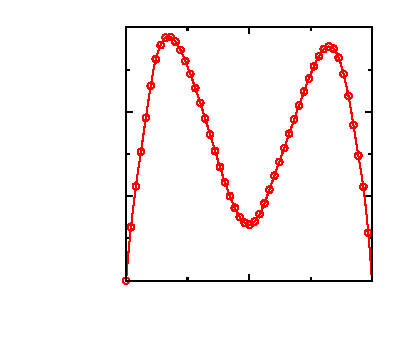
\includegraphics{v_prof_Ra_1e7}}%
    \gplfronttext
  \end{picture}%
\endgroup

        \caption{$\Ra = \num{e7}$}
        \label{fig:vprof_Ra_1e7}
\end{subfigure}\hfill
        \begin{subfigure}{0.5\textwidth}
                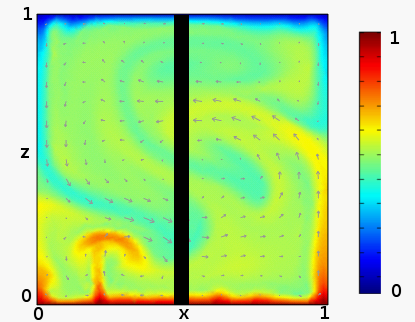
\includegraphics[width=1\textwidth]{Ra_1e7_turbolent.png}
                \caption{Snapshot für $\Ra = \num{e7}$}
                \label{fig:SimSnapshot}
         \end{subfigure}
        \caption{Ergebnisse der numerischen Bestimmung der Geschwindigkeitsprofile für die Rayleighzahlen von $10^{3}$ bis $10^7$. Zu sehen ist das zeitliche Mittel über die Achse durch das Zentrum der Box, wie sie in~(\subref{fig:SimSnapshot}) hervorgehoben ist.
Es wird nur jeder vierte Messwert durch einen Punkt dargestellt. 
        }\label{fig:SimVprof}
\end{figure}


%%%%%%%%%%%%%%%%%%%%%%%%%%%%%%%%%%
% critical rayleigh number 1707
% wikipedia rayleigh benard

%%%%%%%%%%%%%%%%%%%%%%%%%%%%%%%%%%


%	 RAYLEIGH ZAHL DES EXPERIMENTS

% ICH	 SCHATTENPROJEKTION GESCHWINDIGKEIT 

%	 STÖRFREQUENZEN
%		FORMEL

% ICH	 TEMPERATUR ALS ABSTAND DER PLATTE

% ICH	 TEMPERATUR PROFILE

% ICH	 TEMPERATUR DURCH LANGE MESSUNG

%	 GESCHWINDIGKEITSPROFIL DURCH ABBRUCHFREQUENZ

% NUR ICH:
%	GESCHWI VERGlEICH FALL, REIBUNG
%	HISTOGRAMME TEMPERATUR
